\section{Observer}

\begin{figure}[htb]
	\caption{\label{fig_grafico}Estrutura do Observer}
	\begin{center}
	    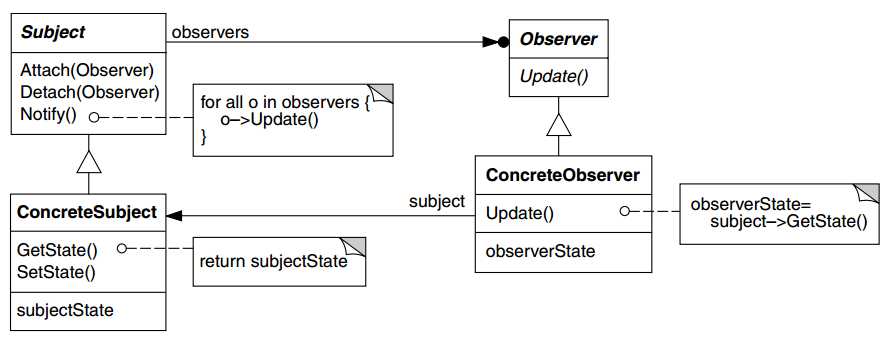
\includegraphics[scale=0.5]{5_padroes-contexto-funcional/5.3_comportamentais/5.3.07_observer/diagram.png}
	\end{center}
\end{figure}

Exemplo Orientado a Objetos:

\begin{lstlisting}[caption={Observer Orientação a Objetos},label=ooobserver]


    
\end{lstlisting}

Contexto Funcional:


\begin{lstlisting}[caption={Observer Funcional},label=fpobserver]
    

    
\end{lstlisting}